\documentclass[a4paper]{article}
\usepackage[T1]{fontenc}
\usepackage[utf8]{inputenc}
\usepackage[margin=1in]{geometry}
\usepackage[english]{babel}
\usepackage{charter}
\usepackage{graphicx}
\usepackage{parskip}
\usepackage{mathtools}
\usepackage{amssymb}
\usepackage{xfrac}
\usepackage{booktabs}
\usepackage{longtable}
\usepackage{hyperref}
\usepackage{tabularx}
\usepackage{booktabs}
\usepackage{makecell}
\usepackage{xcolor}
\hypersetup{
    colorlinks,
    linkcolor={red!50!black},
    citecolor={blue!50!black},
    urlcolor={blue!80!black}
}


\usepackage{setspace} % increase interline spacing slightly
\setstretch{1}

\def\arraystretch{1} % increase tabular cells padding

\title{
\Large{Big Data Analytics 2019}\\
\huge{NY City Taxi Data Analysis}\\
\large{Project}}

\author{
Prof. Marcel Graf\\
Prof. Nastaran Fatemi\\
\\
Romain Claret, Jämes Ménétrey and Damien Rochat\\
MSE Master of Science in Engineering\\
HES-SO University of Applied Sciences and Arts
\date{\today}}

\begin{document}
\maketitle

\tableofcontents
\clearpage

\section{Introduction}
The goal of this project is to identify the busiest areas from New York City, from a taxi agency perspective, in order to open new agency locations, to increase profit, the taxi availability and more globally the customers' satisfaction. This analysis aims to highlight two topics of interest:

\begin{itemize}
    \item Find the best spots to find customers
    \item Identify the most profitable spots (proportional to the longest trips)
\end{itemize}

To help the authors to achieve those objectives and to handle the big data related dataset, they will be using Spark and more specifically PySpark with Dataframes (the Python implementation of Apache Spark), to process the data and perform machine learning.


\section{Dataset}
The dataset, provided by Chris Whong \footnote{The dataset can be found at \url{http://www.andresmh.com/nyctaxitrips/}}, is the list of trips and fares for taxis in New York City, for the year 2013. It is composed of 2 parts, which are themselves fragmented into 12 CSV files, one per month, and for a total of 173'179'759 records.

\begin{itemize}
    \item The trips related information (trip\_data.7z, sized 4.1GB)
    \begin{itemize}
        \item Taxi identification
        \item Start time and end time
        \item GPS coordinates of pick up and drop off
        \item Trip information
    \end{itemize}
    \item The fares related information to each trip (trip\_fare.7z, sized 1.72GB)
    \begin{itemize}
        \item Taxi identification
        \item Start time
        \item Fare information (amount, payment type, tip)
    \end{itemize}
\end{itemize}



\subsection{Structure}
\begin{tabularx}{\textwidth}{XX}
  \toprule
  Data structure of \texttt{trip\_data} & Data structure of \texttt{trip\_fares}\\
  \midrule
    \verb/root/ & \verb/root/\\
    \verb/|- medallion: string/ & \verb/|- medallion: string/\\
    \verb/|- hack_license: string/ & \verb/|- hack_license: string/\\
    \verb/|- vendor_id: string/ & \verb/|- vendor_id: string/\\
    \verb/|- rate_code: string/ & \verb/|- pickup_datetime: timestamp/\\
    \verb/|- store_and_fwd_flag: string/ & \verb/|- payment_type: string/\\
    \verb/|- pickup_datetime: string/ & \verb/|- fare_amount: double/\\
    \verb/|- dropoff_datetime: string/ & \verb/|- surcharge: double/\\
    \verb/|- passenger_count: string/ & \verb/|- mta_tax: double/\\
    \verb/|- trip_time_in_secs: string/ & \verb/|- tip_amount: double/\\
    \verb/|- trip_distance: string/ & \verb/|- tolls_amount: double/\\
    \verb/|- pickup_longitude: string/ & \verb/|- total_amount: double/\\
    \verb/|- pickup_latitude: string/ &\\
    \verb/|- dropoff_longitude: string/ &\\
    \verb/|- dropoff_latitude: string/ &\\
  \bottomrule
\end{tabularx}


\section{Preprocessing}
This section covers the manipulations performed to clean up the data in order to make it eligible to be processed by the machine learning algorithms.

\subsection{Out of bound GPS coordinates}
After visualizing the GPS coordinates on an interactive map, several of the trips were out of the bounds of New York City. They represented about 1.75\% of the trips. As those trips were not related to our objectives, the trips initiated out of NYC were drop in order to keep the clusters' centroids within the city.

\subsection{Invalid fares}
Some of the trip fares were considered invalid; indeed, their values were either null or equal to zero. They represented about 1\% of the records. The fares are used for the second objective, which determines the most profitable spots to set up taxi agencies or pickup spots. Therefore, those records were curated for the second objective.

\section{Machine learning}
The project relied heavily on machine learning for the two objectives. As the first objective is to determine the best locations for building taxi agencies, a good approach is to create customers clusters per region. The centroid of these clusters inherently become the taxi best spots; those clusters are calculated via the K-Means algorithm. The number of clusters required can be hyper-parametered via the value of $k$. The number of clusters depends on how many agencies the taxi company is willing to open. For that purpose, an interval of values have been selected, so the company can review the results and decide their expansion strategy based on what makes more sense.

The second objective is similar to the first one, but it weights the location of the customers with the fares they have paid for the trip.



\subsection{Features selection}
The GPS coordinates represent the fundamental data that are used to determine the centroids of the clusters. Indeed, this project exploits the fact that the means of the GPS locations are meaningful, as they represent coordinates as well and can be plotted on a map. The dataset contains multiple fares values, and it has been decided to sum the \emph{fare\_amount} and the \emph{surcharge}, which correspond to an additional amount such as night period or weekends. An analysis has been performed on the distribution of the sum of fares, in order to alleviate any outliners that can add biases to the results. Figure \ref{fig:distribution-fares-bad} illustrates the histogram of fares over the number of trips. It appears clear that there is a Gaussian distribution at the left of the chart and several heavy outliners distort the result. For that purpose, the maximum amount of fares has been set to 20\$, as it keeps the original form of the Gaussian, as shown in Figure \ref{fig:distribution-fares-capped}. As an interesting fact, the maximum value for the fares is 158'995.8125\$, which does not make much sense as seen on Figure \ref{fig:distribution-fares}.

\begin{figure}
  \centering
  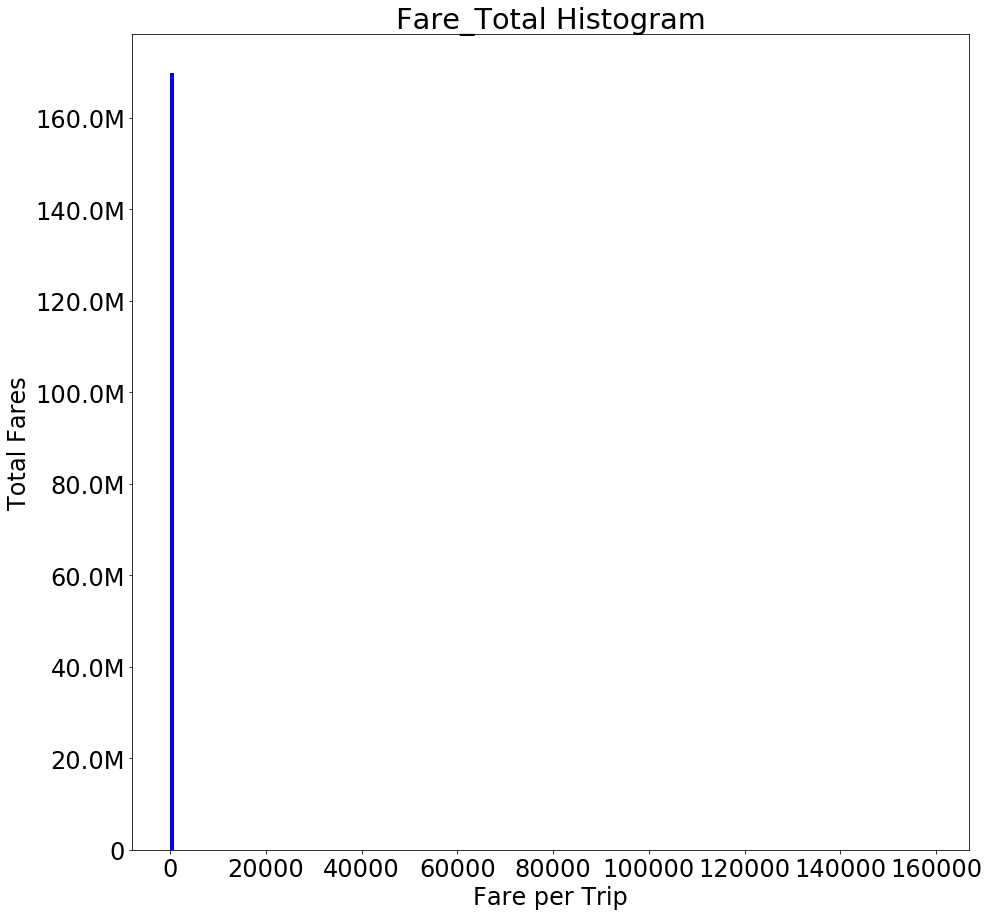
\includegraphics[width=0.6\textwidth]{images/distribution-fares-bad.png}
  \caption{The histogram of the fares over the number of trips.}
  \label{fig:distribution-fares-bad}
\end{figure}

\begin{figure}
  \centering
  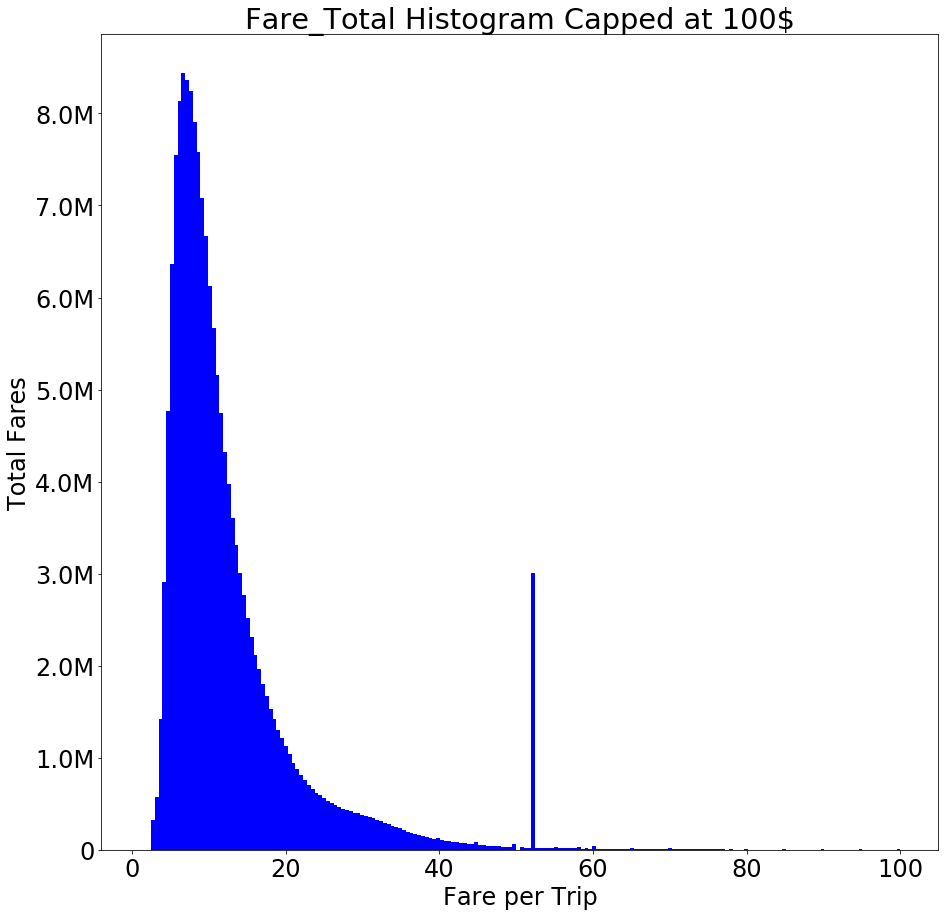
\includegraphics[width=0.6\textwidth]{images/distribution-fares-to-100.png}
  \caption{The histogram of the fares capped at 100\$.}
  \label{fig:distribution-fares-capped}
\end{figure}

\begin{figure}
  \centering
  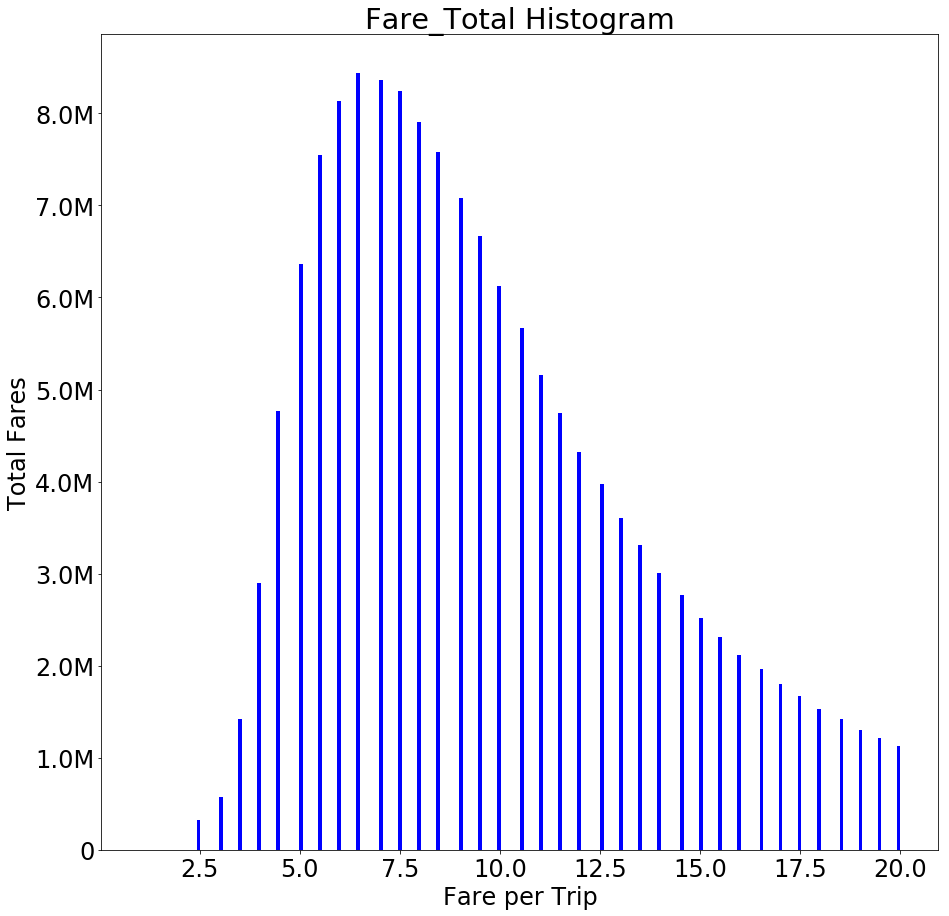
\includegraphics[width=0.6\textwidth]{images/distribution-fares-fix.png}
  \caption{The full histogram of the fares including meaningless values.}
  \label{fig:distribution-fares}
\end{figure}


\subsection{Algorithms}
After several tries over K-Means algorithm hyper-parameters from the PySpark library, the observed that the best performances in for our objectives were the default ones\footnote{\url{https://jaceklaskowski.gitbooks.io/mastering-apache-spark/spark-mllib/spark-mllib-KMeans.html}} . For both objectives, the authors used the same default hyper-parameters, only the $k$ parameter was alternated to generated related clusters. The default parameters tried were listed below:

\begin{itemize}
  \item maxIter=20
  \item initSteps=5
  \item tol=1e-4
\end{itemize}

As we can see in Figure \ref{fig:ml-cpus-max}, it was managed to use the full cpu power the machine used for the machine learning.

\begin{figure}
  \centering
  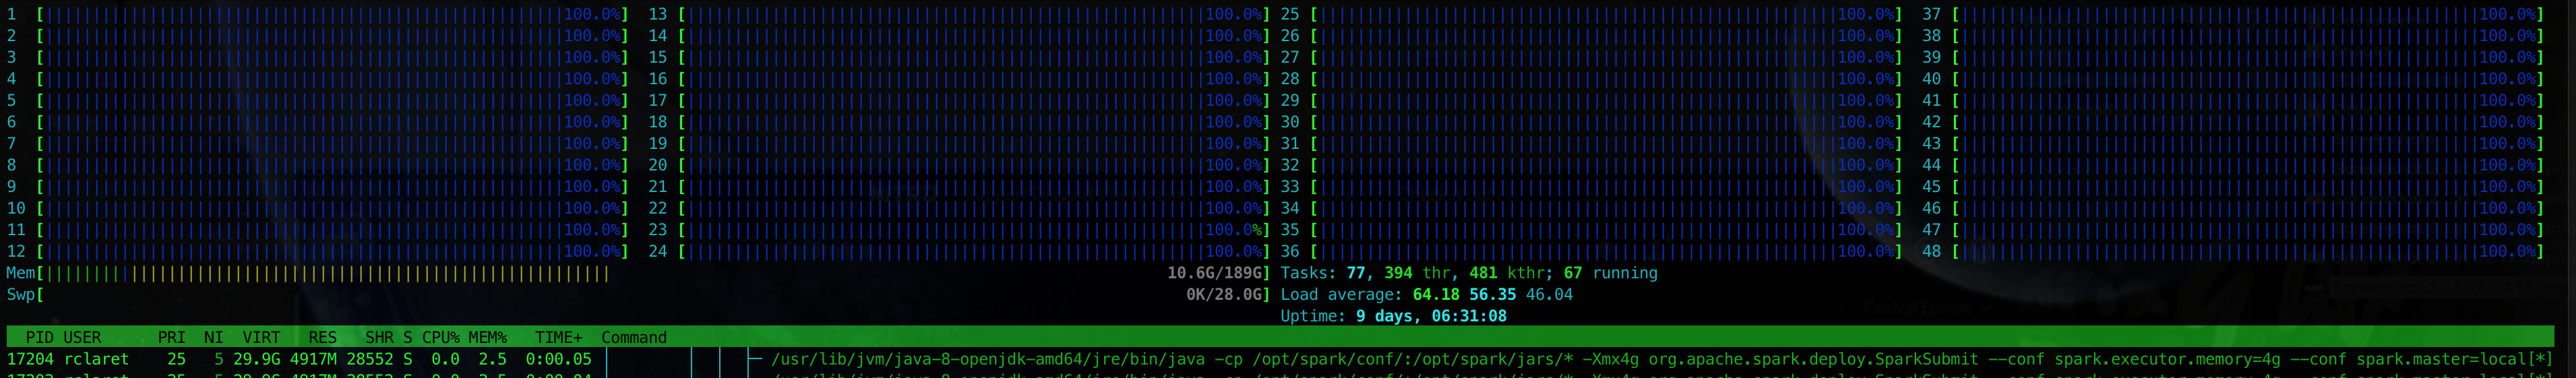
\includegraphics[width=\textwidth]{images/htop-full-cpus.png}
  \caption{\texttt{htop} during training.}
  \label{fig:ml-cpus-max}
\end{figure}

\subsection{Optimizations}
\subsubsection{Sampling the fares}
The computation of the centroids of the second objective has been optimized to take into account the fares of the trips. Indeed, the algorithm of K-means implemented in spark does not provide a way to weight the records differently, based on a value, which would be fair in the case of the project. The intuitive solution to solve this problem is the introduction of the weight notion, which has been accomplished by duplicating each record proportionally of its amount of fares. Following this process, the given records have a stronger attraction to centroids. It is obvious that creating new records proportionally to the number of fares increases the number of records drastically from the initial model, increasing the dataset size of 2'575\%. That size is so large that it took days to compute a single K-means, but the goal of the class, which is "Big Data Analytics" has been fulfilled. \textbf{wink wink}

As a solution to increase the speed of the K-Means clustering, we sampled the fares to circumvent the time and power consumption issues. In a similar process of the music sampling by famous compression algorithms such as MP3, the fares have been grouped by adjacent values and the index of the group has been used instead of the value of the amount, in order to weight in a lighter way the records. We tried the sampling by 3, 4, and 5, and kept the sampling by 3 has it provided the best quality and performance ratio from our perspective. Figure \ref{fig:distribution-fares-sampled} illustrates that the fares have been sampled using three groups. The index of the groups are then used to determine how much time the record must be duplicated, in order to generate to have a stronger gravity.

\begin{figure}
  \centering
  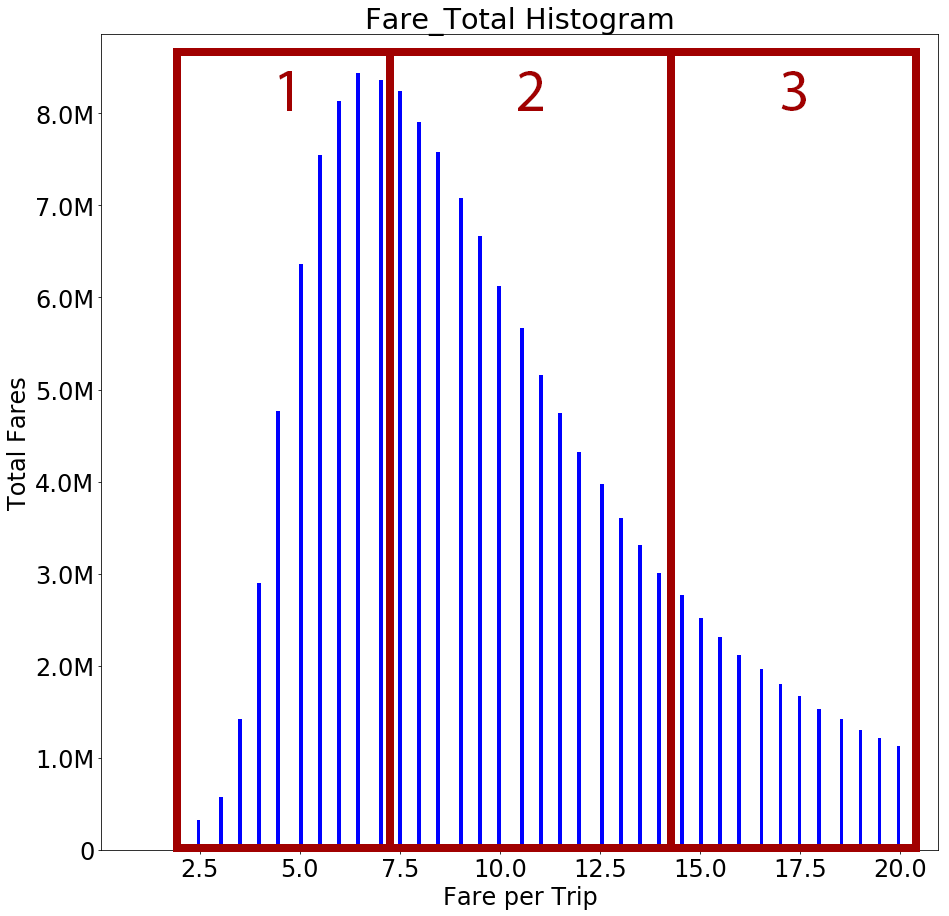
\includegraphics[width=0.6\textwidth]{images/distribution-fares-sampled.png}
  \caption{The sampled distribution of fares using three groups.}
  \label{fig:distribution-fares-sampled}
\end{figure}

The sampling solution\footnote{The source code can be found in the \texttt{src} folder from the project Github repository.} has been implemented in C\#, using the .NET Core application called \emph{DataWalker}. In the workflow, Spark preprocesses the dataset and exports a cleaner dataset into multiple CSV files. The application then reads the files and creates new files with the duplicated records. Finally, the new files are imported in Spark to run the machine learning algorithms. 


\section{Testing and evaluation}
During the making of the project, the authors were confronted with various problems related to data optimization, meta-parametering, and design thinking to provides a meaning out of the dataset.

\subsection{Computation}
Even by following instructions from the class laboratory \textit{Guided lab: Deploy Spark in the Cloud},we were not able to deploy a Spark clusters on AWS via \textit{flintrock}\footnote{\url{https://github.com/nchammas/flintrock}}, the timeouts and versions errors made us stop continuing in this direction.

Luckily, the authors had access to a server dedicated to CPU computation and could use it to run the project on it. However, the Java Virtual Machine and Spark were not friendly all the time while processing, and gave much hard time with errors such as:

\begin{itemize}
    \item java.lang.OutOfMemoryError: Java heap space
    \item Executor heartbeat timed out
    \item Job 74 cancelled because SparkContext was shut down
\end{itemize}

\subsection{Optimization}
Using Big Data datasets implies to think distributed with solutions. However, it also appears that parallelized computations also requires a different strategy to optimize its performances, but most of often its time computation and computer resources consumptions. The authors even implemented custom software to optimize the data transformations to help Spark handle it better.

\subsection{Try, Fails and Meta Parametering}
The whole project could be summarized in this title. Sadly, it does not work out of the box, and the solutions provided had to be state of the art. Requiring much time to spend trying various combinations and optimizations to get the wanted result.

\subsection{Evaluation}
It is hard to evaluate the outcome of the project, but from the authors' point of view, it seems like it is fulfilling the objectives in the most optimized manner that could be found so far.


\section{Results}
The suggested locations for the taxi agencies are depending on the $k$ value, which varies a lot, implying that it is difficult to provide a solution better than another. Indeed, it would depend on the company's strategy for expansion. Thereby, a Web application has been created to visualize the centroids on an interactive map.\footnote{The web application is located at \url{https://zenlulz.github.io/hesso-bigdata-analytics/}.} The view can be adapted using the right pane, which enables the users to select one of the two objectives (by the highest number of customers or by the most profitable spots). The red circles represent the location of the centroids; in other words, the suggested locations for the taxi agencies. Another feature has been implemented to visualize an excerpt of the pickup locations, highlighted by blue circles. Figure \ref{fig:web-app} illustrates the Web application.

As a helper, another C\# application called \emph{GeoJsonParser}\footnote{The source code can be found in the \texttt{src} folder from the Github repository.} was written. Its purpose is to convert the coordinates of SparkML's KMeans clusters' centroids generated into the GeoJSON format supported by the interactive map component \emph{Mapbox}.

\begin{figure}
  \centering
  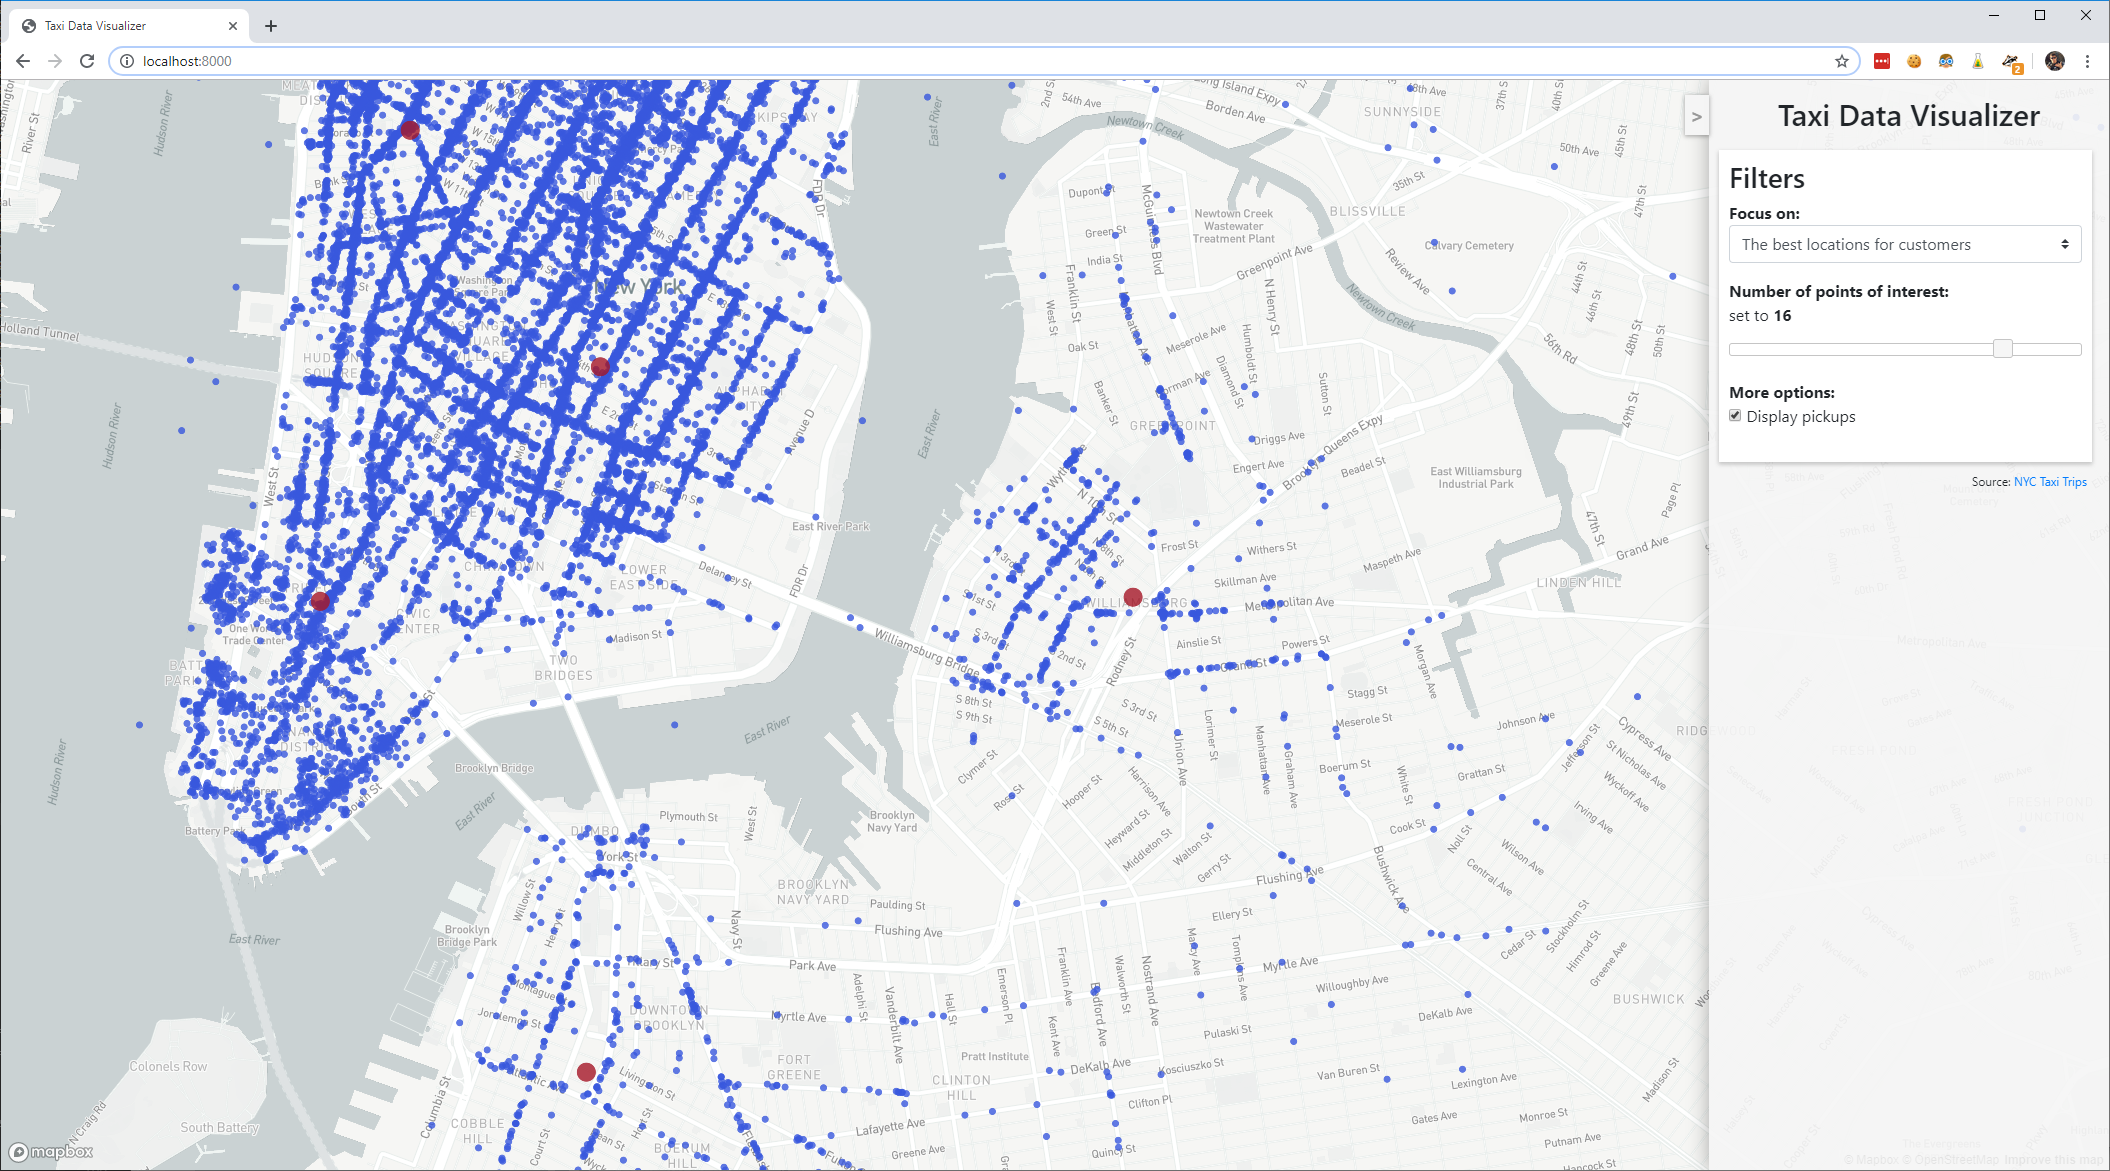
\includegraphics[width=\textwidth]{images/web-app.png}
  \caption{The Web application to visualize the results of the project.}
  \label{fig:web-app}
\end{figure}

\section{Conclusion}
\subsection{Project}
\begin{itemize}
    \item The clusters of customers are also the most profitable
    \item Using Python with PySpark was a good experience
    \item Spark Dataframes are limited compared to the Pandas Dataframes
    \item For specific use-cases, Spark work well out of the box for parallelization
\end{itemize}

\subsection{Personal}
The points that the authors are agreeing on to conclude this project, taking apart that they, of course, enriched their knowledge in the following buzzwords: Big Data Analytics, Spark, Parallelization and Distribution, is that a Big Data Project is a lot of brain's puzzling. Indeed, most of the time, it does not work out of the box, and solutions state of the art are common to solve problems. Optimizing the processing time, without affecting too much the quality of the outcome are meticulous decisions made all the time. Parallelization is not magical, neither is the distribution, having enormous clusters could help, but as an everyday data engineer, it is often not a resource accessible, and tweaks have to be made to get the best outcome out of the available resources. Even with the 48 CPUs server often reached bottlenecks, and the team had to find workarounds to make it work efficiently. One of the solutions was to build custom software to help go through mutual limitations. The design thinking for problem-solving and find strategies were essential to achieve this project.


\subsection{Next steps}
Let keep in mind that this project has been delivered in the academic boundaries and in a restricted time. However, it would be interesting for the authors to see this project evolve. Following are various suggestions to improve the project.

\subsubsection{More processing time}
Providing more computation time to increase the precision of the clusters would be interesting. Indeed, we had to sample our dataset to be able to compute data in the given set of time, which could output less precise outcome.

\subsubsection{Zoom in data}
The dataset is rich, and it would be interesting to use its granularity to look at more details.
\begin{itemize}
    \item On time periods: Days, Weeks, Months, Years
    \item On time groups: Weekday, Weekend, Nights
\end{itemize}

\subsubsection{Prediction}
Do more with machine learning by using algorithms such as Random Forest.
\begin{itemize}
    \item Predict the customers' positions
    \item Predict potential profits at specific spots
\end{itemize}

\subsubsection{More data}
Of course, an interesting point would be to increase the amount of data to extract more features.
\begin{itemize}
    \item Using the full NYC dataset (not only 2013)
    \item Add other taxi services such as UBER
    \item Use of the weather data
\end{itemize}

\subsubsection{Technicalities}
\begin{itemize}
    \item Serializing the data
    \item Try RDD
    \item Compare SparkML and Scikit-Learn
\end{itemize}

\end{document}
























